\documentclass{article}
\pagestyle{empty}
\usepackage{tikz}
\usetikzlibrary{arrows.meta}
\definecolor{diagOrange}{RGB}{240,105,26}
\definecolor{inkGray}{RGB}{51,51,51}
\definecolor{axisGray}{RGB}{138,138,138}
\begin{document}
\noindent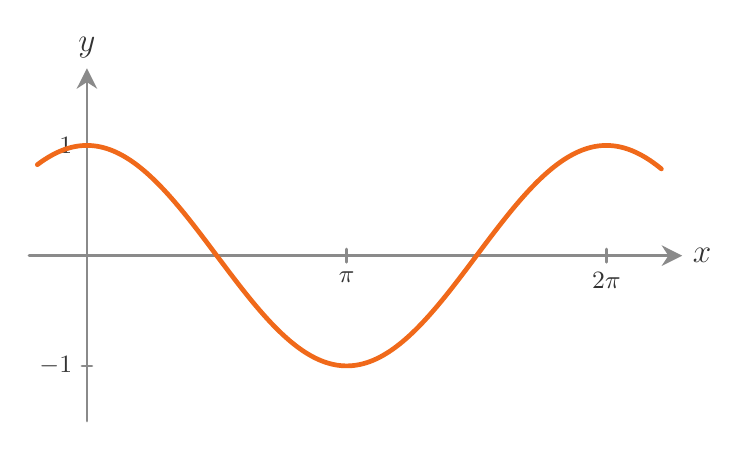
\begin{tikzpicture}[
  x=1.05cm, y=1.4cm,
  >={Stealth[length=2.6mm,width=2.6mm]},
  line cap=round, line join=round,
]
  % axes
  \draw[axisGray, line width=1pt, ->] (-0.7,0) -- (7.2,0)
        node[right, inkGray, font=\sffamily\large] {$x$};
  \draw[axisGray, line width=1pt, ->] (0,-1.5) -- (0,1.7)
        node[above, inkGray, font=\sffamily\large] {$y$};

  % x ticks
  \foreach \tx/\tl in {3.14159/\pi, 6.28319/2\pi}{
    \draw[axisGray, line width=1pt] (\tx,-0.06) -- (\tx,0.06);
    \node[inkGray, font=\sffamily\small, below] at (\tx,-0.06) {$\tl$};
  }
  % y ticks
  \foreach \ty/\tl in {1/1, -1/{-1}}{
    \draw[axisGray, line width=1pt] (-0.06,\ty) -- (0.06,\ty);
    \node[inkGray, font=\sffamily\small, left] at (-0.06,\ty) {$\tl$};
  }

  % curve
  \draw[diagOrange, line width=1.7pt, smooth, samples=120, domain=-0.6:6.95]
        plot (\x, {cos(\x r)});
\end{tikzpicture}
\end{document}
